\documentclass{article}

\author{Stefan Schrijvers, Sven-Bodo Scholz, Thomas Koopman}

\title{Shray: a distributed shared-memory system for array programming}

\usepackage[utf8]{inputenc}
\usepackage{adjustbox}
\usepackage{algorithm}
\usepackage[noend]{algpseudocode}
\usepackage{amsfonts}
\usepackage{amsmath}
\usepackage{amssymb}
\usepackage{amsthm}
\usepackage{booktabs}
\usepackage{caption}
\usepackage{fullpage}
\usepackage{hyperref}
\usepackage{listings}
\usepackage{multicol}
\usepackage{pgfplots}
\usepackage{pgfplotstable}
\usepackage{subcaption}

\DeclareMathOperator{\divi}{div}
\DeclareMathOperator{\md}{~{\mathrm{mod}}~}

\setlength{\parindent}{0pt}
\pgfplotsset{compat=1.17}


    

\begin{document}

\maketitle

\begin{abstract}

A distributed shared memory (DSM) system allows a programmer to treat a distributed memory 
cluster, as a shared memory system. This increases the programmability of clusters. 
We present a DSM library Shray that is tailored to array programming. 

\end{abstract}

\section*{Introduction}

Shray is a distributed shared memory layer tailored for applications operating on arrays.
The API is kept simple so it can be integrated into code-generators. We use the following 
terminology to describe arrays: an $n_1 \times \cdots \times n_d$ array has dimension $d$,
and extent $n_l$ along the $l$th dimension. So 

\[
\begin{pmatrix}
    0 & 1 \\
    2 & 3 \\
    4 & 5 \\
\end{pmatrix}
\]

has dimension two, extent three along the first dimension, and extent two along the second 
dimension.  

\medskip

It builds on the Shray distributed shared memory layer from Andrius Šilinskas'
Bachelor's thesis \cite{Silinskas15}.

\section{Related work}

Volgens mij is er niet zoveel related work. OpenSHMEM is eigenlijk gewoon een RMA library, coarray Fortran komt
er het dichtst bij in de buurt aangezien communicatie impliciet is, maar dat is niet shared-memory.

Samhita \cite{Ramesh11} is a distributed shared memory system implemented in software. It has a more complicated
consistency model that makes it interchangable with pthreads. The downside is that dedicated nodes are necessary 
for storing data and organising the communication.

\section{Design}

The basic idea is as follows. Each processor owns a certain portion of the array. It is only
allowed to write to this portion. A processor can read from the entire array. When an element
is not owned, it is fetched from its owner by Shray. There are several problems that need 
to be overcome:

\begin{itemize}
    \item We need to make checking whether an element is remote or not extremely cheap to 
          not add unacceptable overheads.
    \item Fetching an element from a remote node takes thousands of clock cycles, 
          while a computation may have reciprocal throughput of less than one. 
    \item Memory usage should be scalable.
\end{itemize}

We solve the first two problems by working at page granularity. We protect pages that are 
not owned, so that accessing them raises a segfault. This way we can use the MMU to check 
whether a read is local or not, which is very fast. We then fetch the entire page (or multiple 
pages) to hide the latency. Larger messages also get better bandwidth. 

For the third problem, we implement a cache, with a first-in first-out eviction scheme. 

\medskip

This approach has the same downsides as a physical cache: if there is no locality of reference,
the latency remains as high as when communicating only a single element. It also increases 
bandwidth usage due to the cache line being filled up with elements we do not need. 
Fortunately the same techniques that make an algorithm hardware-cache-friendly, are also 
beneficial for Shray. Most of these techniques such as loop interchange \cite{Allen84}, loop skewing
\cite{Wolfe89}, data reordering, are applicable to array processing.

\section{Consistency model}\label{consistency}

A write to a distributed array $A$ of size $n_1 \times \cdots \times n_d$ at index 
$(i_1, \cdots, i_d)$ is legal, if and only if 
$\texttt{ShrayStart(n1)} \leq i_1 < \texttt{ShrayEnd(n1)}$.

\medskip

A read to a distributed array $A$ is legal, if all writes to $A$ issued before the read, are separated
by an \texttt{ShraySync(A)}, and all writes to $A$ after the read are separated by a 
\texttt{ShrayBarrier} or any \texttt{ShraySync} (not necessarily on $A$ itself). 
This can be useful when reusing an allocation. Suppose \texttt{f(in, out)} reads from in, and writes
to out, and you do not need \texttt{in} afterwards anymore. It is then safe to reuse \texttt{in} after

\begin{lstlisting}
    f(in, out);
    ShraySync(out);
\end{lstlisting}

In addition, reads to a position where we can legally write to are always legal. 
(Because those are local.) That means pointwise operations such as

\begin{lstlisting}
    for (size_t i = ShrayStart(n); i < ShrayEnd(n); i++) {
        for (size_t j = 0; j < n; j++) {
            A[i * n + j] = A[i * n + j] + B[i * n + j]
        }
    }
\end{lstlisting}

is legal, even though the write to \texttt{A[i * n + j]} on the left-hand side is not separated from
the read to \texttt{A[i * n + j]} on the right-hand side.

\section{Optimisation}

In this section we will list some techniques that can be used to improve the performance of the Shray
communication layer. The easiest is to increase the cache-size. This will, until a point, reduce the 
number of times we communicate a certain data element, at the cost of a higher memory consumption. 

\medskip

As mentioned before, another way of improving performance is making the code more cache-friendly. 

\medskip

The last way is specific to a common pattern in array programming: an element-wise reduction. 
This is a situation where an array $A$ is calculated from (large subsets of) distributed arrays, 
at each position. Examples include matrix multiplication, where 

$$C[i_1, i_2] = \sum_{j \in [n]} A[i_1, j] \cdot B[j, i_2]$$

or an n-body simulation where the acceleration at point $i$ is calculated as

$$\sum_{j \in [n]} f(\text{positions}[i], \text{positions}[j])$$ 

for an acceleration function $f$. When we naively let $j$ run from $0$ to $n$, every processor will
access positions and $B$ in the same order. That means the communication is not balanced: first 
all processors request data from the first processor, then the second, etc. It would be better 
if every processor cycled through $[n]$ from a different starting point. Fortunately, this is 
easy to achieve, e.g. by transforming

\begin{lstlisting}
    size_t start = ShrayStart(n);
    size_t end = ShrayEnd(n);
    
    for (size_t i = start; i < end; i++) {
        accel[i].x = 0.0;
        accel[i].y = 0.0;
        accel[i].z = 0.0;
        for (size_t j = 0; j < n; j++) {
            accel[i].x += 
                accelerate(positions[i], positions[j], masses[j]).x;
            accel[i].y += 
                accelerate(positions[i], positions[j], masses[j]).y;
            accel[i].z += 
                accelerate(positions[i], positions[j], masses[j]).z;
        }
    }
\end{lstlisting}

into 

\begin{lstlisting}
    size_t start = ShrayStart(n);
    size_t end = ShrayEnd(n);
    
    for (size_t i = start; i < end; i++) {
        accel[i].x = 0.0;
        accel[i].y = 0.0;
        accel[i].z = 0.0;
        for (size_t j = start; j < n; j++) {
            accel[i].x += 
                accelerate(positions[i], positions[j], masses[j]).x;
            accel[i].y += 
                accelerate(positions[i], positions[j], masses[j]).y;
            accel[i].z += 
                accelerate(positions[i], positions[j], masses[j]).z;
        }
        
        for (size_t j = 0; j < start; j++) {
            accel[i].x += 
                accelerate(positions[i], positions[j], masses[j]).x;
            accel[i].y += 
                accelerate(positions[i], positions[j], masses[j]).y;
            accel[i].z += 
                accelerate(positions[i], positions[j], masses[j]).z;
        }
    }
\end{lstlisting}

This optimisation (in combination with tiling) is used in our implementation of \texttt{nbody}. In languages where this situation can be recognized, the code generator can implement this optimisation. 
An example is SaC \cite{SAC}, where this situation is described by a \texttt{genarray} where every
element is defined using a \texttt{fold} operator.

\section{Results}

\begin{figure}
    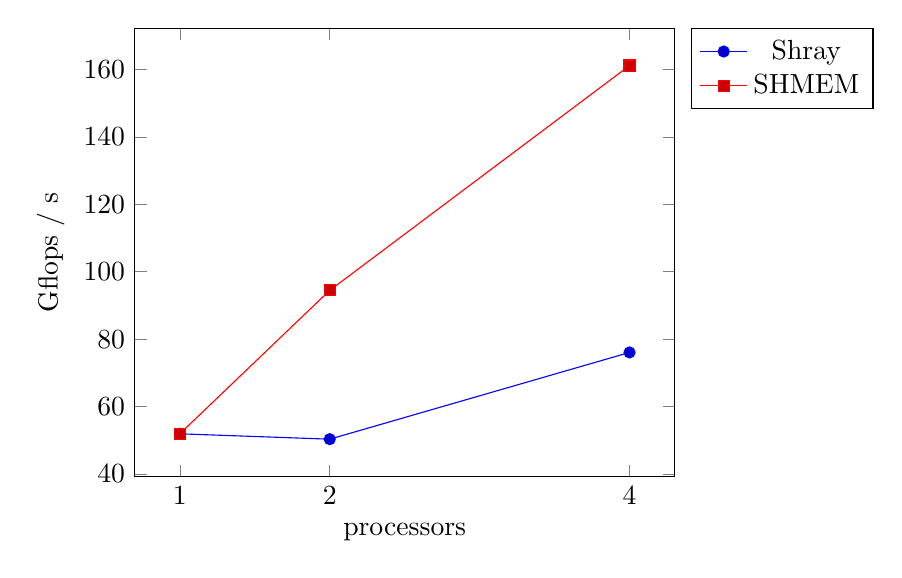
\begin{tikzpicture}
    \begin{axis}[
    xtick = {1, 2, 4},
    xticklabels = {1, 2, 4},
    xlabel=processors,
    ylabel=Gflops / s,
    legend pos = outer north east
    ]
    \addplot table [x = p, y = s] {
    p s
    1 51.934109
    2 50.339479
    4 76.074923
    };
    \addplot table [x = p, y = s] {
    p s
    1 51.934109
    2 94.495071
    4 161.165965
    };
    \legend{Shray, SHMEM}
    \end{axis}
    \end{tikzpicture}
    \caption{Multiplication of two $5000 \times 5000$ matrices}
\end{figure}

oshmem cannot handle this, so for p = 2, took two $4000 \times 4000$ matrices.

Suppose we walk through two arrays in strided fashion, starting at

$f(2t) = a_1 + b_1t$
$f(2t + 1) = a_2 + b2_t$

Now we only look at t multiples of the pagesize, say 4096

\begin{figure}
    \begin{tikzpicture}
    \begin{axis}[
    xtick = {1, 2, 4},
    xticklabels = {1, 2, 4},
    xlabel=processors,
    ylabel=seconds,
    legend pos = outer north east
    ]
    \addplot table [x = p, y = s] {
    p s
    1 3.956
    2 2.449
    4 1.530
    };
%    \addplot table [x = p, y = s] {
%    p s
%    1 
%    2 146.858
%    4 100.624
%    };
    \addplot table [x = p, y = s] {
    p s
    1 3.956
    2 3.399
    4 1.996
    };
    \legend{Shray, coarray Fortran, SHMEM}
    \end{axis}
    \end{tikzpicture}
    \caption{Five iterations on $10000$ bodies. }
\end{figure}

Fortran is much slower. 

\subsection{Predictive prefetching}

This is expensive in logic, but by increasing the cacheline size, that is mitigated. This can be 
helpful for overlapping computation with communication. In common blocking algorithms, like blis's implementation of DGEMM and n-body simulation, we see patterns like: ...

Strided access, interleaved arrays. Pattern may change. Depends on the size of the cacheline.

For nbody we get 3 linear accesses of one part of the array, interleaved with one linear access 
to a different part. That is probably the three accesses to position, and then to masses. For matrix it is pretty consistently two pages. For 2dstencil it is linear.

So as model, suppose we have interleaved strided access to at most ... structures. Can we get dynamically update the cacheline to make the stride equal to one? That is going to be difficult because of alignement issues.

We can keep track of strides by remembering the previous segfault, and taking the difference. Then by also saving the stride, we can keep track of how long we are on that stride. What if we have two interleaved strides, such as

0 1 2 100 3 4 5 101 6 7 8 102 ... ?

We could say if the stride is broken, save the address on a different spot. 
Ignore the difference, and when the stride is broken again, calculate the difference as stride 2.
But this depends on how many interleaved strides there are.

I guess we can keep a stride per allocation, as we have to traverse that anyway and assume we do not have too many allocations.


\section*{Conclusion}

Our results show that a distributed-shared memory layer with fully implicit communication can achieve
performance competitive to hand-coded parallel programs implemented using Coarray Fortran and 
OpenSHMEM, demonstrated with stencil operations, matrix-multiply and an n-body simulation.

\section{Matrix multiply}

Matrix multiply between $m \times n$ matrix $A$ and $n \times k$ matrix $B$ is defined as $(AB)_{ij} = \sum_{l = 1}^{n}a_{il} b_{lj}$. If the elements of $A, B$ are not numbers, but matrices themselves, this still holds, and $a_{jl} b_{lj}$ is matrix multiplication. For example we may consider

\[
A = \begin{pmatrix}
    0 & 1 & 2 & 3 \\
    4 & 5 & 6 & 7 \\
    8 & 9 & 10 & 11 \\
    12 & 13 & 14 & 15 \\
    \end{pmatrix}
\]

as a $2 \times 2$ matrix of $2 \times 2$ matrices, where 

\[
A_{0, 0} = \begin{pmatrix}
    0 & 1 \\
    4 & 5
\end{pmatrix}
\]

This gives some simple parallel algorithms. We can view $A$ as an $p \times 1$ matrix and $B$ as an $1 \times 1$ matrix
to get

\[
AB =
\begin{pmatrix}
A_0 \\
\cdots \\
A_p
\end{pmatrix} B = \begin{pmatrix}
A_0 B \\
\cdots \\
A_p B
\end{pmatrix}
\]

or in words: we can calculate the $s$th chunk of rows of $AB$ by multiplying the sth chunk of rows of $A$ by $B$. 

If we use a block distribution, so processor $s$ owning $A_s$, then accessing $A$ is local. However, the entirety 
of $B$ needs to be loaded in, and this is not memory scalable. So instead we can split up $A$ and $B$ in both directions
to get

\[
A B = \begin{pmatrix}
A_{0, 0} & \cdots & A_{0, p - 1} \\
\vdots & \ddots & \vdots \\
A_{0, 0} & \cdots & A_{0, p - 1} \\
\end{pmatrix} \begin{pmatrix}
B_0 \\
\vdots \\
B_{p - 1}
\end{pmatrix} = \begin{pmatrix}
\sum_{l = 0}^{p - 1} A_{0, l} B_l \\
\vdots \\
\sum_{l = 0}^{p - 1} A_{p - 1, l} B_l
\end{pmatrix}
\]

and then reuse the memory allocated to $B_l$ when calculating $A_{s, l + 1} B_{l + 1}$. This way we only need to allocate a block large enough to hold an $B_l$ at a time, which is memory scalable. (And we can overlap the computation of $A_{s, l} B_l$ with the communication of $B_{l + 1}$, start the sum at different points to balance the communication.) 

\section{Profiling}

If we look at gasnet, we have bandwith of about 7 - 15 GB/s, and latencies of about 1 - 5 $\mu s$. That means
that we can communicate bandwidth wise about $275 - 515 ns$ per page. 
mremap takes about $1 \mu s$ for a single page. For larger blocks of memory this grows, but very slowly. 
Remapping 4MB at once takes about $3 ns$ per page. An AMD Ryzen 3600 can burn through a page in $512 / 50 = 10ns.$

CPU - RAM bandwidth on my AMD Ryzen 3600 is about $9GB/s$, or $450 ns.$ per page. 

\begin{table}[ht]
    \centering
    \begin{tabular}{c|c|c|c}
    Action & time cluster & time Ryzen (Ubuntu 22.10) & time single node EDUcluster \\
    \hline
    Bandwidth (large chunks) & 275 - 515 & 450 & 275 \\
    Bandwidth (single page) & 800 - 2000 & &  \\
    Latency & 1000 - 5000 & 14 & 14 \\
    mremap (1 page) & & 1000 & 560 \\
    mremap (1000 pages) & & 3 & 4 \\
    segfault + mprotect & & 4500 - 6500 & 3600 \\
    mprotect (1 page) & & 650 & 219 \\
    mprotect (1000 pages) & & 0.3 & 0.1 \\
    vfmadd213pd (on ymm registers) & 10 & 10 & 10\\
    munmap/mmap free (1 page) & & 2000 & 650 \\
    munmap/mmap free (1000 pages) & & 2 & 1    
    \end{tabular}
    \caption{Time in ns per page. Measurements taken on a six-core AMD Ryzen CPU (2019),
    the educluster on a single shared memory node, 
    and several clusters (before 2018, by Gasnet).}
    \label{tab:my_label}
\end{table}

vfmadd213pd is the instruction with the highest flop throughput on amd64. Latency on Ryzen was measured using

\begin{lstlisting}
sudo modprobe eeprom 
decode-dimms
\end{lstlisting}

\section{Heap structure}

Our cache is a list of

\begin{lstlisting}
struct {
    void *address;
    size_t size;
};
\end{lstlisting}

elements. Together with a \texttt{size\_t usedMemory}. Define functions

\begin{lstlisting}[language=C]
/* Waits until all communication is complete. */
void waitLoaded(void);
/* Releases elements from the cache, until we have decreased usedMemory 
 * by at least size. */
void evict(size_t size);
/* For each element line in the cache, release 
 * [line.address, line.address + line.size] \cap [address, address + size] */
void evictPrecise(void *address, size_t size); 
/* Does an unblocking fetch on [address, address + size[, adds 
 * numberOfPages to usedMemory. */
void triggerLoad(void *address, size_t size);
\end{lstlisting}

Can we make sure no entries overlap? Then we do not have to search the entire list for precise eviction. 

On a segfault we check whether it is because of PROT\_WRITE or PROT\_NONE (I hope this is possible). If PROT\_WRITE we just wait until the fetches are complete, PROT\_READ the memory and return. If PROT\_NONE we 

Can we check why something segfaults? If so, we can tell immediately whether a fetch is in progress by seeing it is
write protected, or not fetched at all by seeing it is PROT\_NONE'd.  

\bibliographystyle{plain}
\bibliography{refs.bib}

\end{document}
